\documentclass[Main]{subfiles}
\begin{document}

\section{Background and vision}
The customer, Aarhus University, wants a system to handle submissions from students in the course, ITDMAT.

The lecturer will assign handins for the students who in return will submit handins in small groups to each other.
The students retrieve a list of people to assign handins to and another list of students to review.
When a student has reviewed another, the student must send a mail to the lecturer and the reviewed student.
\\
\\
This process result in a lot of mails to the lecturer and they are not written from any template.
To handle this, a system has been ordered to keep track of students handins, reviews and deadlines of these.

\begin{figure}
	\centering
	\begin{subfigure}[b]{0.6\textwidth}
		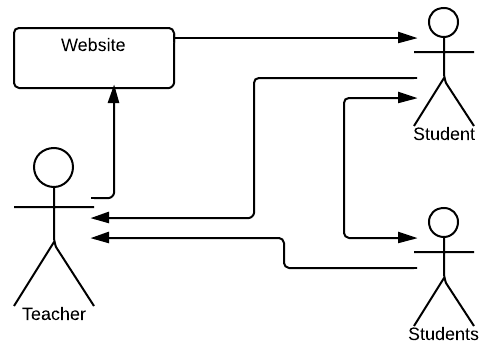
\includegraphics[width=\textwidth]{Overview-old}
		\caption{The old system}
		\label{fig:overview-old}
	\end{subfigure}%

	\begin{subfigure}[b]{0.6\textwidth}
		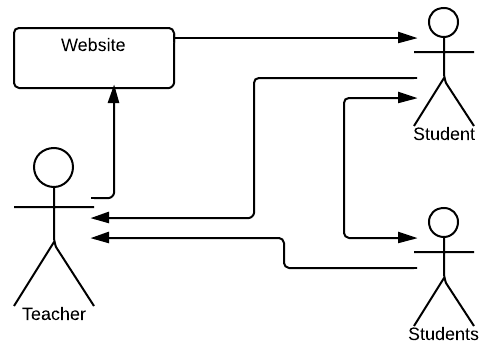
\includegraphics[width=\textwidth]{Overview-old}
		\caption{The new system}
		\label{fig:overview-new}
	\end{subfigure}
	\caption{The old and the new system requested}\label{fig:overview}
\end{figure}


\end{document}